\documentclass[a4paper]{article}
\usepackage[english]{babel}
\usepackage[utf8]{inputenc}
\usepackage{fancyhdr}
\usepackage{hyperref}
\usepackage{amsmath,amsfonts,amssymb,amsthm}
\usepackage[a4paper, bottom=1.3in, top=1.3in, right=1in, left=1in]{geometry}
\usepackage[usenames,dvipsnames]{xcolor}
\usepackage[lined,boxed]{algorithm2e}
\usepackage{natbib}
\usepackage{tikz}
\usepackage{wrapfig}
\usepackage{subcaption}

\usetikzlibrary{calc}
\definecolor{amaranth}{rgb}{0.9, 0.17, 0.31}
\newcommand{\rcol}[1]{{\color{amaranth}#1}}

\newcommand{\wh}[1]{\widehat{#1}}
\newcommand{\wt}[1]{\widetilde{#1}}
\newcommand{\transp}{\intercal}

%%%%%%%%%%%%%%%%%%%%%%%%%%%%%%%%%%%%%%%%%%%
% Insert your name here
\newcommand{\fullname}{Raphael Reme}
%%%%%%%%%%%%%%%%%%%%%%%%%%%%%%%%%%%%%%%%%%%

\newcommand{\lecture}[3]{
   \pagestyle{myheadings}
   \thispagestyle{plain}
   \newpage
   \setcounter{page}{1}
   \noindent
   \begin{center}
   \framebox{
      \vbox{\vspace{2mm}
              \hbox to .97\textwidth { {\bf MVA: Reinforcement Learning (2020/2021) \hfill Homework 2} }
       \vspace{6mm}
       \hbox to .97\textwidth { {\Large \hfill #1 \hfill } }
       \vspace{6mm}
       \hbox to .97\textwidth { {Lecturers: \it A. Lazaric, M. Pirotta  \hfill {{\footnotesize(\today)}}} }
      \vspace{2mm}}
   }
   \end{center}
   Solution by {\color{amaranth}\fullname}
   \markboth{#1}{#1}
   \vspace*{4mm}
}


\DeclareMathOperator*{\argmax}{\arg\,\max}
\DeclareMathOperator*{\argmin}{\arg\,\min}
\DeclareMathOperator*{\arginf}{\arg\,\inf}


\setlength{\parindent}{0cm}
\begin{document}
\lecture{Approximate Reinforcement Learning}{1}


\pagestyle{fancy}
\fancyhf{}
\rhead{Full name: {\color{amaranth}\fullname}}
\lhead{(Approximate) Reinforcement Learning}
\cfoot{\thepage}

\textbf{Instructions}
\begin{itemize}
    \item The deadline is \textbf{December 21, 2020. 23h00}
    \item By doing this homework you agree to the \emph{late day policy, collaboration and misconduct rules} reported on \href{https://piazza.com/class/kf86owfvi2u2lg?cid=8}{Piazza}.
    \item \textbf{Mysterious or unsupported answers will not receive full credit}.
          A correct answer, unsupported by calculations, explanation, or algebraic work will receive no credit; an incorrect answer supported by substantially correct calculations and explanations might still receive partial credit.
    \item Answers should be provided in \textbf{English}.
\end{itemize}


\section{TRPO}
Compare Conservative Policy Iteration (\url{https://people.eecs.berkeley.edu/~pabbeel/cs287-fa09/readings/KakadeLangford-icml2002.pdf}) and TRPO (\url{https://arxiv.org/abs/1502.05477}). Highlight similarities and differences.

\subsection*{Answers}
First the Trust Region Policy Optimization (TRPO) is much more recent and is based on the Conservative Policy Iteration (CPI). They both
design an algorithm for policy optimization and their goal is to improve the stability/monotony of this optimization process.

In CPI they define a policy advantage function that allows to compare two policy given a initial distribution. And they use it with an epsilon greedy policy
chooser to check whether they are making progress or not. This allows to be more confident in the learning process.

Whereas in TRPO instead of checking that the algorithm is improving, they define an area where the policy should improve and a surrogate function to
optimize. The resolution of this constrained optimization problem gives the next best policy in this area. And the formulation of the problem ensure a
better monotony in the learning process.

\section{Linear TD}
Consider the Linear TD(0) algorithm. Given a tuple $(s_t, a_t, s_{t+1}, r_t)$ such that $s_{t+1} \sim p(\cdot| s_t,a_t)$ with $a_t \sim  \pi$ and $r_t \sim r(s_t, a_t)$, the TD update rule is given by
\begin{align*}
    \theta_{t+1} = \theta_t + \alpha \Big(r_t + \gamma \phi_{t+1}^\transp \theta_t - \phi_t^\transp \theta_t\Big) \phi_t
\end{align*}
where $\phi_t = \phi(s_t)$ and $\alpha_t \geq  0$.
We ask to characterize the expected behavior of the steps taken by the TD algorithm in ``steady state''.
Let $A = \mathbb{E}[\phi_t(\phi_t  - \gamma \phi_{t+1})^\transp]$ and $b = \mathbb{E}[r_t \phi_t]$ be the steady state matrices, where the expectation is such that $s_t \sim d^{\pi}$, $s_{t+1} \sim p(\cdot| s_t, a_t)$,  $a_t \sim \pi(\cdot|s_t)$. Note that $d^{\pi}$ is the stationary distribution of policy $\pi$.
\begin{enumerate}
    \item Write the expected updated $\mathbb{E}[\theta_{t+1}| \theta_t]$ as a function of  $A$ and $b$. If the process converges, what is the fixed point?
    \item If correctly derive, you should notice that $A$ plays a central role in the stability of the update. If  $A$ is positive definite, $\theta_t$ shrinks at every update. Given the definition of $A$ show that $A = \Phi^\transp D (I - \gamma P) \Phi$ for appropriate matrices.
    \item Given this decomposition show that $A$ is positive definite.\\
          Hints: 1) Any matrix $M$ is positive definite if and only if the symmetric matrix $S = M + M^\transp$ is positive definite.
          2) Any symmetric real matrix $S$ is positive definite if all of its diagonal entries are positive and greater
          than the sum of the absolute values of the corresponding off-diagonal entries.
\end{enumerate}
This shows that the TD(0) update is stable in the stationary regime. Additional conditions and steps are necessary to prove convergence.


\paragraph{Off-policy learning.}
Often we have access to a large amount of data collected through a set of different policies, called behavioral policies.
The objective will be to use these samples to compute the value function of a target policy $\pi$. For simplicity suppose that we have a single behavioral policy $\rho \neq \pi$.
The off-policy Linear TD(0)~\citep{PrecupSD01} is simply
\begin{align}\label{eq:offtdlin}
    \theta_{t+1} = \theta_t + \alpha \boldsymbol{w_t} \Big(r_t + \gamma \phi_{t+1}^\transp \theta - \phi_t^\transp \theta_t\Big) \phi_t
\end{align}
where $w_t = \frac{\pi(a_t|s_t)}{\rho(a_t|s_t)}$ is the importance weight.

\begin{itemize}
    \item Consider the following MDP with $2$ states and $2$ actions
          \begin{center}
              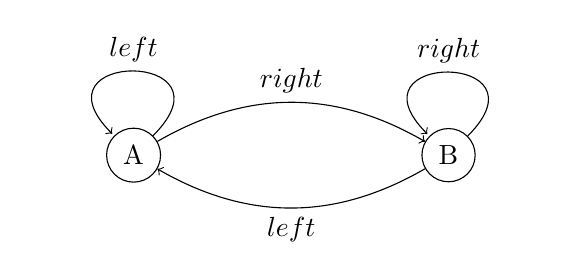
\begin{tikzpicture}
                  \node[circle, draw] (A) at (0,0) {A};
                  \node[circle, draw] (B) at (4,0) {B};
                  \path[->] (A) edge[bend left] node[above] {$right$} (B);
                  \path[->] (B) edge[bend left] node[below] {$left$} (A);
                  \path[->] (B) edge[loop] node[above] {$right$} (B);
                  \path[->] (A) edge[loop] node[above] {$left$} (B);
              \end{tikzpicture}
          \end{center}
          Consider a behavioral policy $\rho(right| \cdot) = 1/2$ and a target policy $\pi(right|\cdot) = 1$.
          The reward function is $0$ everywhere and the value function is parametrized through a single parameter $\theta$ such that $V(A)= 0.8\theta$ and $V(B) = 2\theta$.
          Show that the update~\eqref{eq:offtdlin} diverges. Assume that $\theta_t = 10$, $\alpha = 0.1$ and $\gamma =0.9$.
\end{itemize}

\subsection*{Answers}
\subsubsection*{2.1}
\begin{equation*}
    \begin{aligned}
        \mathbb{E}[\theta_{t+1}|\theta_t] & = \mathbb{E}\left[\theta_t + \alpha \left(r_t + \gamma \phi_{t+1}^\transp \theta_t - \phi_t^\transp \theta_t\right) \phi_t\right]                                                                                          \\
                                          & = \theta_t + \alpha \mathbb{E}\left[r_t \phi_t\right] - \alpha \mathbb{E}\left[(\phi_t - \gamma \phi_{t+1})^\transp \theta_t \phi_t \right]                                                                                \\
                                          & = \theta_t + \alpha b - \alpha \mathbb{E}\left[ \phi_t (\phi_t - \gamma \phi_{t+1})^\transp \theta_t \right]                                & \text{(Because $(\phi_t - \gamma \phi_{t+1})^\transp \theta_t$ is a scalar)} \\
                                          & = \theta_t + \alpha b - \alpha \mathbb{E}\left[ \phi_t (\phi_t - \gamma \phi_{t+1})^\transp\right] \theta_t                                                                                                                \\
                                          & \boxed{= (I - \alpha A) \theta_t + \alpha b}
    \end{aligned}
\end{equation*}

If the process converges then the fixed point $\theta$ verifies:
\begin{equation*}
    \begin{aligned}
        \mathbb{E}[\theta|\theta] & = (I - \alpha A) \theta + \alpha b                                               \\
        \alpha A \theta           & = \alpha b                                                                       \\
        A \theta                  & = b                                & \text{(The case $\alpha=0$ is irrelevant.)} \\
    \end{aligned}
\end{equation*}
This is a linear system, which can be solve using the moore-penrose inverse of a matrix:
\begin{equation*}
    \theta \in \Bigg\{ \begin{aligned}
         & \emptyset                   &  & \text{if $AA^+b \neq b$} \\
         & \{A^+ b + (I - A^+A)w, w \} &  & \text{otherwise}         \\
    \end{aligned}
\end{equation*}

If $A$ is invertible, then $\boxed{\theta = A^{-1}b}$.

\subsubsection*{2.2}

\begin{equation*}
    \begin{aligned}
        A & = \mathbb{E}\left[ \phi_t (\phi_t - \gamma \phi_{t+1})^\transp \right]                                                                                         \\
          & = \mathbb{E}\left[ \phi(s_t) (\phi(s_t) - \gamma \phi(s_{t+1}))^\transp \right]                                                                                \\
          & = \sum_{s, s'} \mathbb{P}(s, s') \phi(s) (\phi(s) - \gamma \phi(s'))^\transp                                                                                   \\
          & = \sum_{s, s'} \mathbb{P}(s)\mathbb{P}(s'|s) \phi(s) (\phi(s) - \gamma \phi(s'))^\transp                                                                       \\
          & = \sum_{s, a, s'} \mathbb{P}(s)\mathbb{P}(s', a|s) \phi(s) (\phi(s) - \gamma \phi(s'))^\transp                                                                 \\
          & = \sum_{s, a, s'} d^\pi(s) \pi(a|s) p(s'|s, a) \phi(s) (\phi(s) - \gamma \phi(s'))^\transp                                                                     \\
          & = \sum_{s, a, s'} d^\pi(s) \pi(a|s) p(s'|s, a) \phi(s) \phi(s)^\transp - \gamma \sum_{s, a, s'} d^\pi(s)\pi(a|s)p(s'|s, a) \phi(s) \phi(s')^\transp            \\
          & = \sum_{s} d^\pi(s) \phi(s) \phi(s)^\transp \sum_{a, s'} \pi(a|s) p(s'|s, a) - \gamma \sum_{s, s'} d^\pi(s) \phi(s) \sum_a \pi(a|s)p(s'|s, a) \phi(s')^\transp \\
          & = \sum_{s} d^\pi(s) \phi(s) \phi(s)^\transp - \gamma \sum_{s, s'} d^\pi(s) \phi(s) \sum_a \pi(a|s)p(s'|s, a) \phi(s')^\transp                                  \\
    \end{aligned}
\end{equation*}
Let's defined the matrix $\Phi = \begin{pmatrix}
        \phi(s_0)^\transp \\
        \vdots            \\
        \phi(s_n)^\transp \\
    \end{pmatrix}$.\\
And the diagonal matrix $D = (\delta_{ss'}d^\pi(s))_{s, s'}$ and $P = (\sum_a \pi(a|s)p(s'|s, a))_{s, s'} = (\mathbb{P}(s'|s))_{s, s'}$. Then we have:
\begin{equation*}
    \begin{aligned}
        A & = \sum_{s, s'} D_{s,s'} \phi(s) \phi(s')^\transp - \gamma \sum_{s, s'} D_{s,s} \phi(s) P_{s, s'} \phi(s')^\transp \\
          & = \Phi^\transp D \Phi - \gamma (\Phi^\transp D) P \Phi                                                            \\
          & \boxed{= \Phi^\transp D (I - \gamma P) \Phi}
    \end{aligned}
\end{equation*}

\subsubsection*{2.3}

First, we will assume that $(\phi_i)_i$ are choosen such that they form an independent family and such that $\Phi$ is injective. (If it was not,
it would exists $\theta$ and $\theta$ such that $V = \Phi\theta = \phi\theta'$ which is not at all what we want. And moreover with $\Phi$ non injective, then
$A$ cannot be positive definite.)\\
With this assumption, $A$ is positive definite if and only if $D(I - \gamma P)$ is positive definite, and this is equivalent to:
$M = D (I - \gamma P) + (I - \gamma P^\transp)D = 2D - \gamma DP - \gamma P^\transp D$ is positive definite. We can now use the 2nd hint as $M$ is symmetric:
\begin{equation*}
    \begin{aligned}
        \forall s \in S, \sum_{s' \neq s} |M_{s, s'}| & = \sum_{s' \neq s} |2D_{s, s'} - \gamma DP_{s, s'} - \gamma P^\transp D_{s, s'}|                                                                             \\
                                                      & = \sum_{s' \neq s} |0 - \gamma d^\pi(s) \mathbb{P}(s'|s) - \gamma d^\pi(s') \mathbb{P}(s|s')|                                                                \\
                                                      & = \gamma \sum_{s' \neq s} d^\pi(s) \mathbb{P}(s'|s) + \gamma \sum_{s' \neq s} d^\pi(s') \mathbb{P}(s|s')                                                     \\
                                                      & = \gamma d^\pi(s) (1 - \mathbb{P}(s|s)) + \gamma \sum_{s' \neq s} d^\pi(s') \mathbb{P}(s|s')             & \text{(Because $\sum_{s'} \mathbb{P}(s'|s) = 1$)} \\
                                                      & = \gamma d^\pi(s) (1 - \mathbb{P}(s|s)) + \gamma (d^\pi(s) - d^\pi(s)\mathbb{P}(s|s))                    & \text{($d^\pi$ is the stationnary distribution)}  \\
                                                      & = 2\gamma d^\pi(s) - 2\gamma d^\pi(s)\mathbb{P}(s|s))                                                                                                        \\
                                                      & \le 2 d^\pi(s) - 2\gamma d^\pi(s)\mathbb{P}(s|s))                                                        & (0 < \gamma < 1)                                  \\
                                                      & \le 2 D_{s, s} - \gamma DP_{s, s} - \gamma P^\transp D_{s, s}                                                                                                \\
                                                      & \le M_{s, s}                                                                                                                                                 \\
    \end{aligned}
\end{equation*}
Therefore $M$ is positive definite and so is $A$!

\subsubsection*{2. Off-policy learning}
First let's show that the stationnary policy $d^\rho(.) = \frac{1}{2}$.\\
As $d^\rho$ is stationnary:
\begin{equation*}
    d^\rho(s') = \sum_{s, a} d^\rho(s) \rho(a | s) p(s'| s, a) = \frac{1}{2} \sum_s d^\rho(s) \sum_a p(s'| s, a)
\end{equation*}
But in our environment $\forall s, s' \sum_a p(s'| s, a) = 1$ (Indeed the environment is deterministic and from each state there is an unique action
leading to any other state). Therefore:
\begin{equation*}
    d^\rho(s') = \frac{1}{2} \sum_s d^\rho(s) = \frac{1}{2}
\end{equation*}
Now let's consider $\phi$: As $V(s) = \phi(s)\theta$, we have $\phi(A) = 0.8$ and $\phi(B) = 2)$.

Finally let's compute $\mathbb{E}_\rho(\theta_{t+1}|\theta_t)$:
\begin{equation*}
    \begin{aligned}
        \mathbb{E}_\rho(\theta_{t+1}|\theta_t) & = \theta_t + \alpha \mathbb{E}_\rho( w_t \phi_t (0 + \gamma \phi_{t+1} - \phi_t) )\theta_t                                                                                        \\
                                               & = \theta_t \left(1 + \alpha \sum_{s, a, s'} d^\rho(s) \rho(a|s) p(s'|a, s) \frac{\pi(a|s)}{\rho(a|s)} \phi(s) (\gamma \phi(s') - \phi(s))\right)                                  \\
                                               & = \theta_t \left(1 + \frac{\alpha}{2} \sum_{s, a, s'} \pi(a|s) p(s'|a, s) \phi(s) (\gamma \phi(s') - \phi(s))\right)                                                              \\
                                               & = \theta_t \left(1 + \frac{\alpha}{2} \sum_{s, s'} p(s'|right, s) \phi(s) (\gamma \phi(s') - \phi(s))\right)                                     & \text{(As $\pi(left|s)=0$)}    \\
                                               & = \theta_t \left(1 + \frac{\alpha}{2} \sum_{s} \phi(s) (\gamma \phi(B) - \phi(s))\right)                                                         & \text{(As $p(A|right, s)= 0$)} \\
                                               & = \theta_t \bigg(1 + \frac{\alpha}{2} \Big(\phi(A) (\gamma \phi(B) - \phi(A)) + \phi(B) (\gamma \phi(B) - \phi(B)) \Big)\bigg)                                                    \\
                                               & \boxed{= 1.02 \times \theta_t}
    \end{aligned}
\end{equation*}
Therefore the update diverges.

\section{REINFORCE}
In class we have seen the derivation of the policy gradient theorem in the ``Monte-Carlo style''. Recall that the policy gradient is given by
\[
    \nabla_\theta J(\pi_\theta) = \mathbb{E}_{\tau \sim \mathbb{P}(\cdot|\pi_\theta)}\left[ \nabla_\theta \log \mathbb{P}(\tau|\pi_\theta)
        R(\tau)
        \right]
\]
where $R(\tau) = \sum_{t=1}^{|\tau|} r_t$. % and $b(\tau)$ is a baseline.

\begin{itemize}
    \item By construction the policy gradient is on-policy. Derive an off-policy variant by assuming to collect samples from a behavioral policy $\mu(s,a)$. The target policy, i.e., the policy for which we want to compute the gradient is $\pi_{\theta}$
\end{itemize}

So far we have seen the ``Monte Carlo'' derivation of the gradient.
It is possible to derive the gradient theorem by leveraging the recursive structure of the Bellman equation. Recall that for a $\gamma$-discounted infinite-horizon MDP, we define the policy performance $J(\pi_\theta) = \mathbb{E}\left[\sum_{t=1}^{+\infty} \gamma^{t-1} r_t | s_1 \sim \rho, \pi_\theta \right]$. Then, the policy gradient is given by
\begin{align}
    \label{eq:pgt}
    \nabla_\theta J(\theta) = \mathbb{E}_{s \sim d^{\pi_\theta}} \mathbb{E}_{a \sim \pi_\theta(s, \cdot)}
    \left[
        \nabla_{\theta} \log \pi_\theta(s,a) Q^\pi(s,a)
        \right]
\end{align}
where $d^{\pi_\theta}(s) = \lim_{T \to \infty} \sum_{t=1}^{T} \gamma^{t-1} \mathbb{P}(s_t=s|\pi,s_1 \sim \rho)$.

\begin{itemize}
    \item Derive the gradient in Eq.~\ref{eq:pgt}. \emph{Hint: you can start from $V^{\pi}(s) = \sum_a \pi(s,a) Q^{\pi}(s,a)$}
\end{itemize}

\subsection*{Answers}
\subsubsection*{3.1}
Let's $\tau$ a trajectory: $\tau =  (s_0, a_0, s_1, a_1, \dots, s_{T+1})$.\\
We have $\mathbb{P}(\tau | \pi) = p(s_0) \times \pi(a_0 | s_o) \times p(s_1|s_0, a_0) \times \dots \times p(s_{T+1} | s_T, a_T) = C \times \prod_{t=0}^T \pi(a_t|s_t)$.
With C a constante w.r.t the policy $\pi$.\\
Therefore, with two different policy, $\mu$ and $pi$,
$\frac{\mathbb{P}(\tau | \pi)}{\mathbb{P}(\tau | \mu)} = \frac{C \times \prod_{t=0}^T \pi(a_t|s_t)}{C \times \prod_{t=0}^T \mu(a_t|s_t)} = \prod_{t=0}^T \frac{\pi(a_t|s_t)}{\mu(a_t|s_t)} = w_{\pi, \mu}(\tau)$\\
Now let's compute $\nabla_\theta J(\pi_\theta)$ using an off-policy $\mu$:
\begin{equation*}
    \begin{aligned}
        \nabla_\theta J(\pi_\theta) & = \mathbb{E}_{\tau \sim \mathbb{P}(\cdot| \pi_\theta)}\left[ \nabla_\theta \log \mathbb{P}(\tau|\pi_\theta)R(\tau)\right]                             \\
                                    & = \int_\tau \mathbb{P}(\tau|\pi_\theta) \nabla_\theta \log \mathbb{P}(\tau|\pi_\theta)R(\tau) d\tau                                                   \\
                                    & = \int_\tau \mathbb{P}(\tau|\mu) \frac{\mathbb{P}(\tau|\pi_\theta)}{\mathbb{P}(\tau|\mu)} \nabla_\theta \log \mathbb{P}(\tau|\pi_\theta)R(\tau) d\tau \\
                                    & = \int_\tau \mathbb{P}(\tau|\mu) w_{\pi_\theta, \mu}(\tau) \nabla_\theta \log \mathbb{P}(\tau|\pi_\theta)R(\tau) d\tau                                \\
                                    & \boxed{= \mathbb{E}_{\tau \sim \mathbb{P}(\cdot|\mu)}\left[ w_{\pi_\theta, \mu}(\tau) \nabla_\theta \log \mathbb{P}(\tau|\pi_\theta)R(\tau)\right]}   \\
    \end{aligned}
\end{equation*}


\subsubsection*{3.2}

First let's rewrite $J(\pi_\theta)$ with the value function:
\begin{equation*}
    \begin{aligned}
        J(\pi_\theta) & = \mathbb{E}\left[\sum_{t=1}^{+\infty} \gamma^{t-1} r_t | s_1 \sim \rho, \pi_\theta \right]                                                                          \\
                      & = \sum_{(s_t, a_t)_{t \ge 1}} \rho(s_1) \prod_{t \ge 1} \pi_\theta(a_t|s_t) \prod_{t \ge 1} p(s_{t+1}|s_t, a_t) \sum_{t=1}^{+\infty} \gamma^{t-1} r_t                \\
                      & = \sum_{s_1} \rho(s_1) \sum_{(s_{t+1}, a_t)_{t \ge 1}} \prod_{t \ge 1} \pi_\theta(a_t|s_t) \prod_{t \ge 1} p(s_{t+1}|s_t, a_t) \sum_{t=1}^{+\infty} \gamma^{t-1} r_t \\
                      & = \mathbb{E}_{s \sim \rho}\left[ \mathbb{E}\left[\sum_{t=1}^{+\infty} \gamma^{t-1} r_t | s_1 = s, \pi_\theta \right]\right]                                          \\
                      & = \mathbb{E}_{s \sim \rho}\left[ V^{\pi_\theta}(s) \right]                                                                                                           \\
    \end{aligned}
\end{equation*}
We have therefore $\nabla_\theta J = \mathbb{E}_{s \sim \rho}\left[ \nabla_\theta V^{\pi_\theta}(s) \right]$.\\
Let's compute $\nabla_\theta V^{\pi_\theta}(s)$ using that $V^{\pi_\theta}(s) = \sum_a \pi_\theta(s, a) Q^{\pi_\theta}(s, a)$ and
$Q^{\pi_\theta}(s, a) = r(s, a) + \gamma \sum_{s'} p(s'|s, a) V^{\pi_\theta}(s')$:

\begin{equation*}
    \begin{aligned}
        \nabla_\theta V^{\pi_\theta}(s) & = \sum_a \nabla_\theta \pi_\theta(s, a) Q^{\pi_\theta}(s, a) + \sum_a \pi_\theta(s, a) \nabla_\theta Q^{\pi_\theta}(s, a)                                                                   \\
                                        & = \sum_a \pi_\theta(s, a) Q^{\pi_\theta}(s, a) \nabla_\theta \log \pi_\theta(s, a) + \sum_a \pi_\theta(s, a) \left(0 + \gamma \sum_{s'} p(s'|s, a) \nabla_\theta V^{\pi_\theta}(s') \right) \\
                                        & = \mathbb{E}_{a \sim \pi_\theta(s, \cdot)}[Q^{\pi_\theta}(s, a) \nabla_\theta \log \pi_\theta(s, a)] + \gamma \sum_{s'} p(s'|s, \pi_\theta) \nabla_\theta V^{\pi_\theta}(s')                \\
    \end{aligned}
\end{equation*}
\vspace{10px}

Let's use matrix notation: $G = (\nabla_\theta V^{\pi_\theta}(s))_s$,
$T = \left(\mathbb{E}_{a \sim \pi_\theta(s, \cdot)}[Q^{\pi_\theta}(s, a) \nabla_\theta \log \pi_\theta(s, a)]\right)_s$ and\\
$P = \left(\sum_a \pi_\theta(s, a) p(s'|s, a) \right)_{s, s'} = (p(s'| s, \pi_\theta))_{s, s'}$.
\vspace{10px}

We can then write:
\begin{equation*}
    G = T + \gamma PV\\
\end{equation*}
\begin{equation*}
    (I - \gamma P)G = T\\
\end{equation*}
\vspace{10px}

We could show that $\sum_{t=1}^\infty \gamma^{t-1} P^{t-1}$ is well defined and then\\
$\sum_{t=1}^\infty \gamma^{t-1} P^{t-1} (I - \gamma P) = \sum_{t=1}^\infty \gamma^{t-1} P^{t-1} - \sum_{t=2}^\infty \gamma^{t-1} P^{t-1} = I$.\\
Thus $G = \sum_{t=1}^\infty \gamma^{t-1} P^{t-1} T$.
\vspace{10px}

Moreover we have: $p(s_t = s' | s_1 \sim \rho, \pi_\theta) = \sum_s \rho(s) p(s_t = s' | s_1 = s, \pi_theta) = \sum_s \rho(s) P^{t-1}_{s', s}$.
($P$ is the transition matrix.)

Finally:
\begin{equation*}
    \begin{aligned}
        \nabla_\theta J(\theta) & = \mathbb{E}_{s \sim \rho}\left[ \nabla_\theta V^{\pi_\theta}(s) \right]                  \\
                                & = \mathbb{E}_{s \sim \rho}\left[ G_s \right]                                              \\
                                & = \sum_s \rho(s) G_s                                                                      \\
                                & = \sum_s \rho(s) \sum_{s'} \sum_{t=1}^\infty \gamma^{t-1} P^{t-1}_{s, s'} T_{s'}          \\
                                & = \sum_{s'} \sum_{t=1}^\infty \gamma^{t-1} \sum_s \rho(s) P^{t-1}_{s', s} T_{s'}          \\
                                & = \sum_{s'} \sum_{t=1}^\infty \gamma^{t-1} p(s_t = s' | s_1 \sim \rho, \pi_\theta) T_{s'} \\
                                & = \sum_{s'} d^{\pi_\theta}(s') T_{s'}                                                     \\
                                & = \mathbb{E}_{s \sim d^{\pi_\theta}} T_s                                                  \\
                                & \boxed{= \mathbb{E}_{s \sim d^{\pi_\theta}} \mathbb{E}_{a \sim \pi_\theta(s, \cdot)}
        \left[\nabla_{\theta} \log \pi_\theta(s,a) Q^\pi(s,a)\right]}                                                       \\
    \end{aligned}
\end{equation*}


\begin{wrapfigure}{r}{0.4\textwidth}
    \centering
    \includegraphics[width=.4\textwidth]{images/networks}
    \caption{DQN network (left) and partial Dueling DQN (right).}
    \label{fig:net}
    \vspace{-50pt}
\end{wrapfigure}


\section{DQN}
The goal of this exercise is to compare different variants of Deep Q-Learning (a.k.a. DQN).

\paragraph{DQN.} Recall from the class the DQN aims to minimize the following loss function
\[
    L(\theta) = \mathbb{E}_{s,a,r,s' \sim \mathcal{D}} \left[
        \left(
        r + \gamma \max_{a' \in\mathcal{A}} Q(s',a';\theta') - Q(s,a; \theta)
        \right)^2
        \right ]
\]
where $\theta'$ is the parameter of the target network updated every $C$ iterations from $\theta$.
\begin{enumerate}
    \item (written) This objective resembles a classical supervised learning problem. Could you highlight the differences?
    \item (written) Could you describe the role of $C$ and the trade-off at play in choosing a good value for $C$?
\end{enumerate}


\vspace{.2in}
\emph{Replay Memory.} As we play, we store our transitions $(s, a, r, s')$ in a buffer $\mathcal{D}$. Old examples are deleted as we store new transitions. To update our parameters, we sample a minibatch from the buffer and perform a stochastic gradient descent update.

\vspace{.2in}
\emph{$\epsilon$-greedy exploration.} For exploration, we use an $\epsilon$-greedy strategy. It is standard to use a linear annealing schedule from $\epsilon_{start}$ to $\epsilon_{\min}$.

\vspace{.2in}
\emph{Q-function representation.} As suggested in the original paper, the Q-function is represented using a neural network with input a state $s$ and output a vector of dimension $|\mathcal{A}|$ containing the estimated Q-value for each action $a \in \mathcal{A}$.
\begin{enumerate}
    \item (written) What is one benefit of representing the Q function as $Q(s; \theta) \in \mathbb{R}^{|\mathcal{A}|}$?
\end{enumerate}

Implementation
\begin{enumerate}
    \item (code) Implement DQN. We provided an almost complete version of DQN in \texttt{dqn\_start.py.py}.
          Implement the network on Fig.~\ref{fig:net}(left).
\end{enumerate}
The code generates two plots. The first plot shows the performance (cumulative reward) over the learning process (i.e., as a function of time steps). The second figure shows the performance of the associated greedy policy on a test environment averaged over multiple episodes.\footnote{Usually, this metric is evaluated less frequently since it is more computationally costly. It is a parameter in the code. By default we run every 2 episodes.} It also saves the results in a file called \texttt{dqn\_results.txt}.
\begin{enumerate}
    \item (code) A single run is not enough to evaluate the performance of an algorithm. To have significant results, we need to perform multiple repetitions. Change the code to run multiple versions of DQN and reports the average performance and uncertainty as function of time steps (for both figures). We provide a script that reads files generated by \texttt{dqn\_start.py.py} that can be used to generate the requested figures.\footnote{It is not necessary to use this script to generate figures.}
\end{enumerate}

\paragraph{Competitors.} We would like to evaluate DQN with newer variants of DQN, namely Double DQN and Dueling DQN.
In class we have seen the principle of Double DQN while we refer to the original paper for Dueling DQN (\url{https://arxiv.org/abs/1511.06581}).

The difference between DQN and Double DNQ is how the target network is built. In Double DQN we use the greedy action suggested by $Q(s,a; \boldsymbol{\theta})$ to evaluate the target (i.e., $\theta'$), see the appendix of \url{https://arxiv.org/abs/1511.06581}.
In Dueling DQN, the Q function is estimated as
\[
    Q(s,a) = V(s) + A(s,a) - \frac{1}{|\mathcal{A}|} \sum_{a'} A(s,a')
\]
$V$ and $A$ share parameters.
Dueling DQN can be implemented ``standard'' or ``double''.

Starting from the code of \texttt{dqn\_start.py.py},
\begin{enumerate}
    \item (code) Implement Double DQN. Use the same network of DQN.
    \item (code) Implement Dueling Double DQN. See Fig.~\ref{fig:net} for the network with shared parameters.
    \item Compare the performance of the algorithms
\end{enumerate}

\subsection*{Answers}
\subsubsection*{4.1-4.2}
The main difference with classical supervised learning is that the target depends on the trained network. Indeed the target is $r + \gamma max_{a'} Q(s', a')$
and $Q$ is computed with the network that we are training. It leads to some issues as we try to fit something that changes during the training! This is why
we use the C constant. It allows us to keep the target steady for some iterations with the introduction of a second network: the target network. (another big
difference with classical supervised learning) This network
is only updated each C iterations (it will then load the parameters of the main trained network.) and is used to compute the target. Having a high C will
grant more stability to the training. But with a high C we will focus on training towards an outdated target for too long.

Another difference comes from the dataset. First, the dataset is generated from what we have learnt, which is rarely the case in supervised learning.
Moreover, at a certain point in training it will forget part of the dataset replacing former transitions with new ones (In particular the random exploration
of the beginning). Therefore the network will from time to time forgets that some basic actions are wrong as they are no longer in the dataset
(because the network don't take them anymore) and will retry them. It can be a good thing (if the environment is random, or evolves) but it also leads to
huge drop in performance from time to time. (which does not really occur in supervised learning where the dataset is often constant.)

\subsubsection*{4.3}
Representing the Q function as a function of state with learnable parameters $\theta$ allows us to keep in memory only a limited amount of
parameters instead of trying to approximate this function for each state and action (like in tabular case). Moreover there is no need to discretise the state space
with this representation. And as we are using a continuous function (neural network) close states will have close Q values
(which is what we expect in this environment!)

\subsubsection*{Results}

\begin{figure}[h!]
    \centering
    \begin{subfigure}[b]{0.4\linewidth}
        \includegraphics[width=\linewidth]{images/dqn_l}
    \end{subfigure}
    \begin{subfigure}[b]{0.4\linewidth}
        \includegraphics[width=\linewidth]{images/dqn_t}
    \end{subfigure}
    \caption{DQN performances}
    \label{fig:dqn}
\end{figure}

\begin{figure}[h!]
    \centering
    \begin{subfigure}[b]{0.4\linewidth}
        \includegraphics[width=\linewidth]{images/ddqn_l}
    \end{subfigure}
    \begin{subfigure}[b]{0.4\linewidth}
        \includegraphics[width=\linewidth]{images/ddqn_t}
    \end{subfigure}
    \caption{Double DQN performances}
    \label{fig:ddqn}
\end{figure}


\begin{figure}[h!]
    \centering
    \begin{subfigure}[b]{0.4\linewidth}
        \includegraphics[width=\linewidth]{images/dddqn_l}
    \end{subfigure}
    \begin{subfigure}[b]{0.4\linewidth}
        \includegraphics[width=\linewidth]{images/dddqn_t}
    \end{subfigure}
    \caption{Dueling Double DQN performances}
    \label{fig:dddqn}
\end{figure}

The three algorithms have very similar results. They all reach maximum rewards after around 6000 steps. We can nonetheless notice that the Double DQN
greedy policy seems more stable at the end of the training. And that the Dueling Double DQN greedy policy is even more stable all along the training.

But we do not observe significative improvements in rewards for this environment. (We can't as the simplest method already reached the best performance
possible)

\bibliographystyle{plainnat}
\bibliography{bibliography}
\end{document}